\documentclass{beamer}
\usepackage{graphicx}
\usepackage{hyperref}
\title{CPP Community Garden Meeting Note}
\author{An Pham, Myriam}
\institute{Calpoly Pomona}
\date{August 15, 2023}
\usetheme{Boadilla}
%\usetheme{Berkeley}
\usepackage{graphicx}
\usepackage{booktabs}
\usepackage{hyperref}
\usepackage[english]{babel}

\begin{document}
\frame{\titlepage}

\begin{frame}
\frametitle{Overview}
\begin{enumerate}
  \item  Discuss data aggregation.
   \item Decide the testing procedure to assure data integrity.
   \item Address LoraWAN to stakeholders to support IoT large scale deployment.
   \item Architecture Differences.
   \item Potential Developement. 
 \end{enumerate}
\end{frame}

\begin{frame}
  \frametitle{When do we aggregate sensor data?}
  \begin{itemize}
        \item Additional json attribute requirement may arise. NOTE: ecowitt doesn't provide location info.
    \item Naming the farming zone based on the moisture sensor radius coverate. 
    \item Shift the data modifying process to local before sending it to the cloud to avoid extra cost or overrelying on lambda function. (optional)
  \end{itemize}
 \end{frame}

\begin{frame}
  \frametitle{Sensors Test}
  \begin{itemize}
    \item Find out tests that can run against data.
      \begin{itemize}
        \item Regression Testing (consolidate with data team). 
	\item Different moisture sensors would have different measurement. How to solve this?
      \end{itemize}
  \end{itemize}
\end{frame}

\begin{frame}[t]
  \frametitle{Estitimate on the Cost of Moisture Sensors}
  \framesubtitle{Wihout solar cost}

  \begin{figure}[h]

  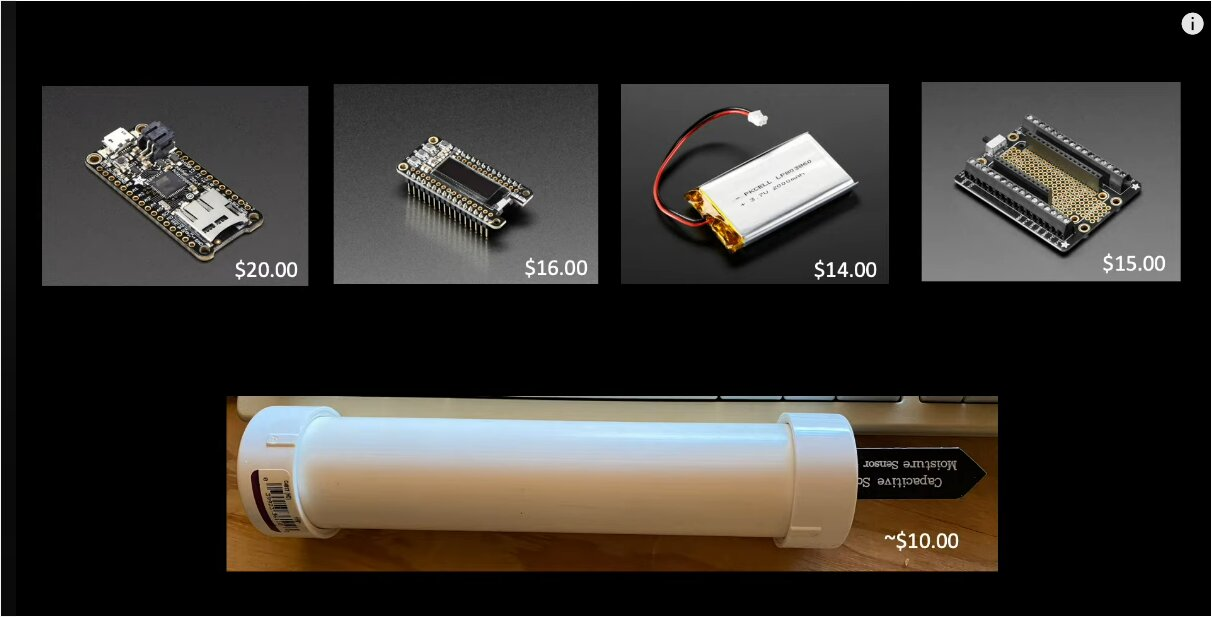
\includegraphics[scale=0.15]{modest-make-soil-moisture-irrigration.jpg}

    \caption{Example of moisture sensor component (Source: Modest Maker)}
\end{figure}

\end{frame}



\begin{frame}
  \frametitle{Architecture Differences with selected criteria}
  \begin{itemize}
    \item Understand the correlation of bandwith and power consumption.
      \begin{itemize}
        \item sensors are end devices in Lora network.
	\item reduce the transmitting size would reduce power consumption. 
	\item how long does it take to send one message of LoraWAN?
	\item Seperate the Sensors Network from the could. The Cloud shoud be last mileage component.
      \end{itemize}
  \end{itemize}
\end{frame}

\begin{frame}[t]
  \frametitle{How does Lora fit in with OSI network stack}
  \begin{figure}[h]
  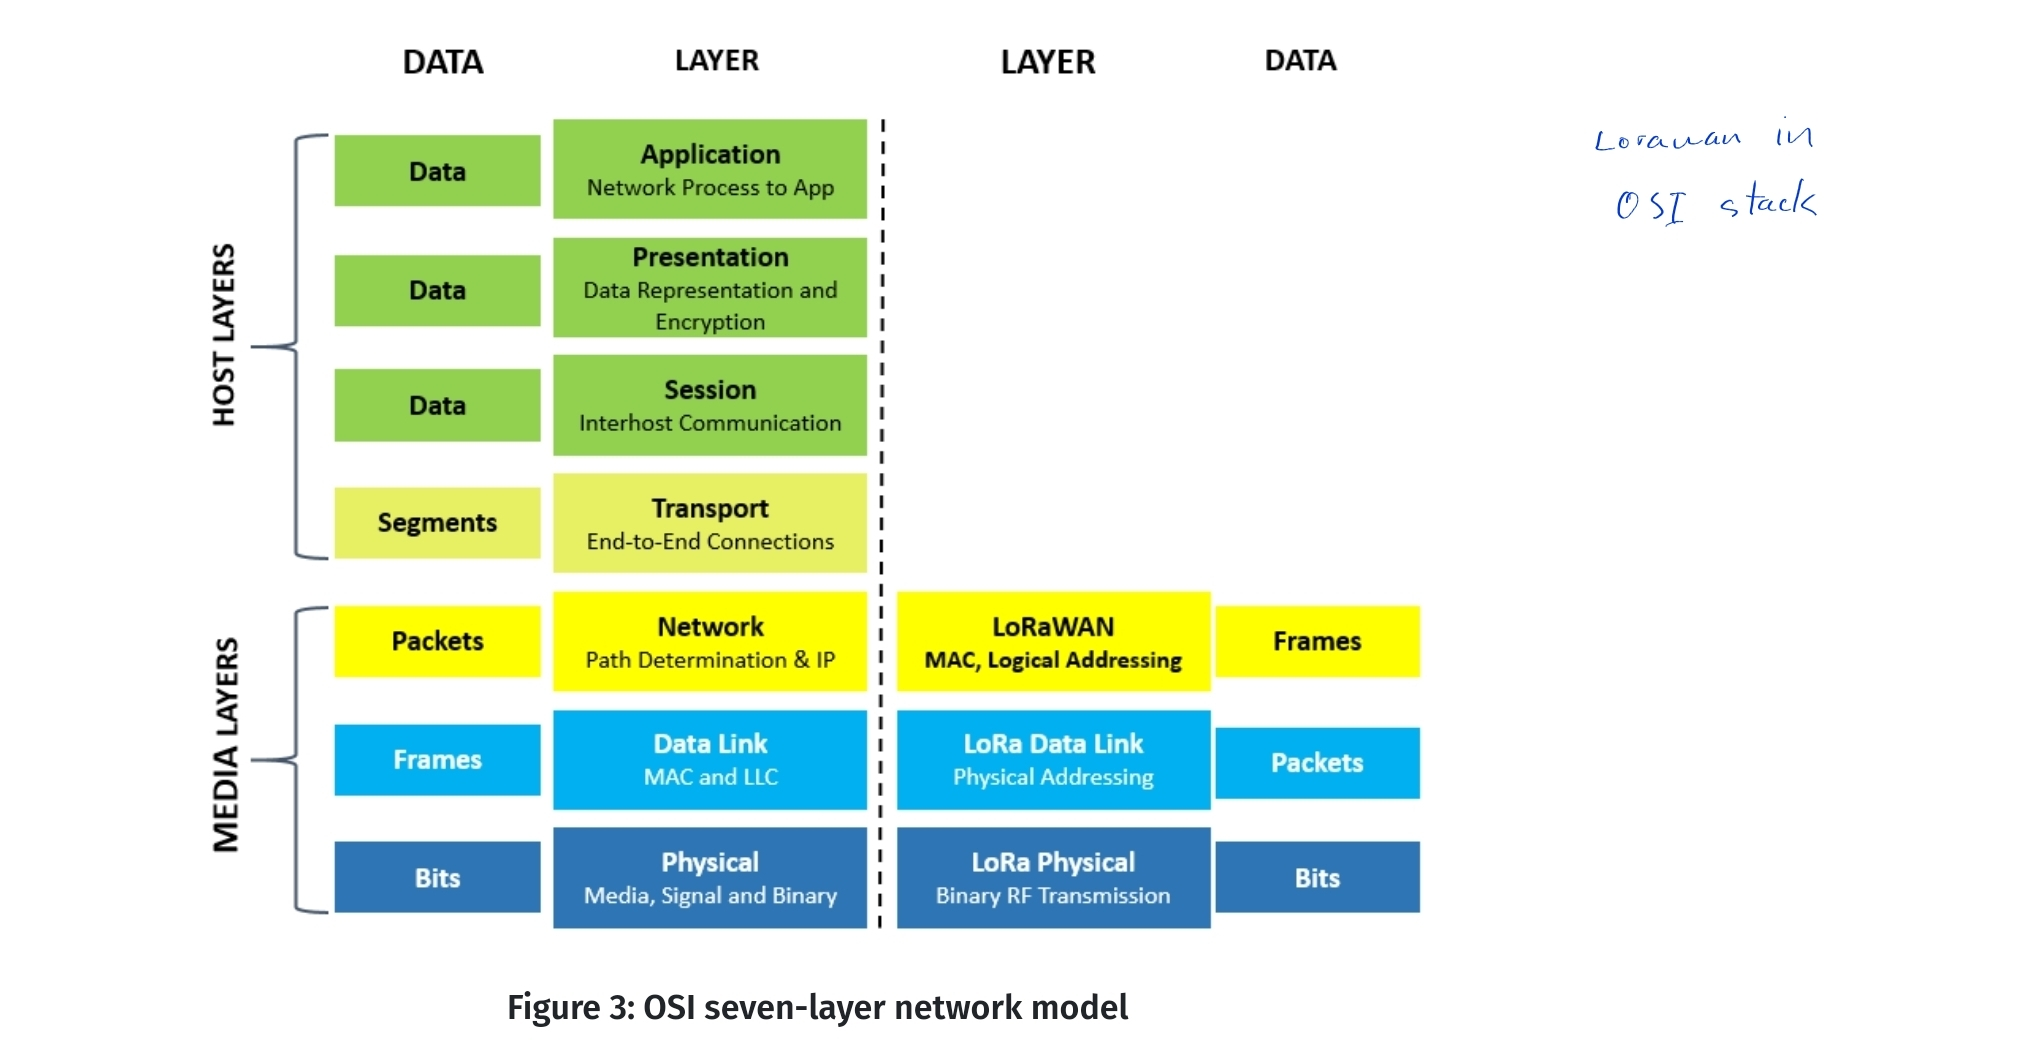
\includegraphics[scale=0.15]{osi-model-lora.jpg}
    \caption{Lora in OSI stack (Source: SEIMEN Lora IOT)}
\end{figure}
\end{frame}


\begin{frame}
  \frametitle{Components of LoraWAN network}
  \begin{itemize}
    \item LoraWAN Gateway.
    \item Virtual Lora Network (can be hosted on raspberry pi or AWS).
    \item End Device type (refer to device classification)
  \end{itemize}
\end{frame}
  
\begin{frame}
  \frametitle{How to Build One?}
  \framesubtitle{What include:}
  \begin{figure}
  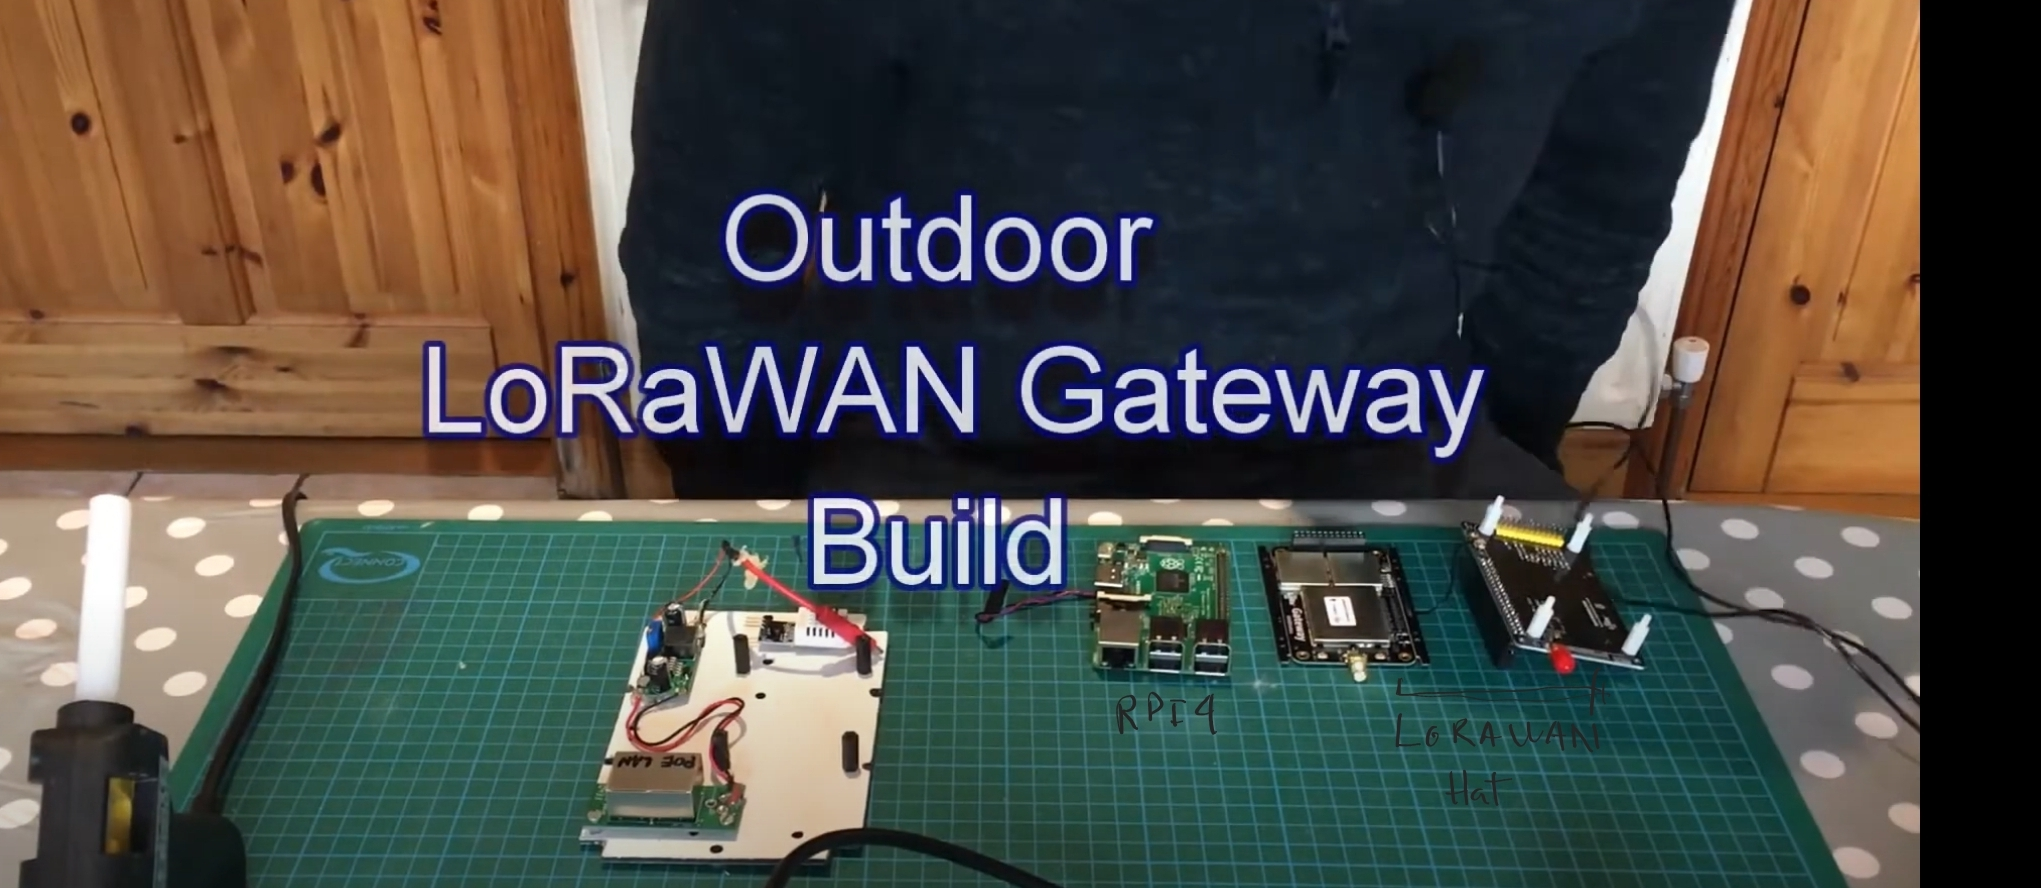
\includegraphics[scale=0.15]{outdoor-lorawan-gateway.jpg}
  \end{figure}
\end{frame}


\begin{frame}[t]
  \frametitle{End Device Classification}
 \begin{itemize}
   \item Classification based on the payload bandwith of end device send to gateway.
   \item It reflects the interval of data transfer. 
   \item In short, there are three types of lora end devices.
     \begin{itemize}
       \item Class A: sending and receiving message within 2s (required low latency connection with the cloud)
       \item Class B: receiving mode only, used for pump control only accept downlink messages.
       \item Class C: deeper sleeping cycle, every 5s device wake up to listen to receiving messages.
     \end{itemize}
 \end{itemize} 
\end{frame}

\begin{frame}[t]
  \frametitle{Key Benefits of Lora IoT Deployment}
  \begin{itemize}
    \item Reduce the cost of hardware on the field.
    \item Thus reduce the cost to power them.
    \item Utilize right message sending cycle.
    \item Open-source and fully developed with AWS IoT Core. Refer to \url{https://docs.aws.amazon.com/iot/latest/developerguide/connect-iot-lorawan.html} AWS IoT Core for LoraWAN.
  \end{itemize}
\end{frame}

\begin{frame}[t]
  \frametitle{Key Benefits cont.}
  \begin{center}
  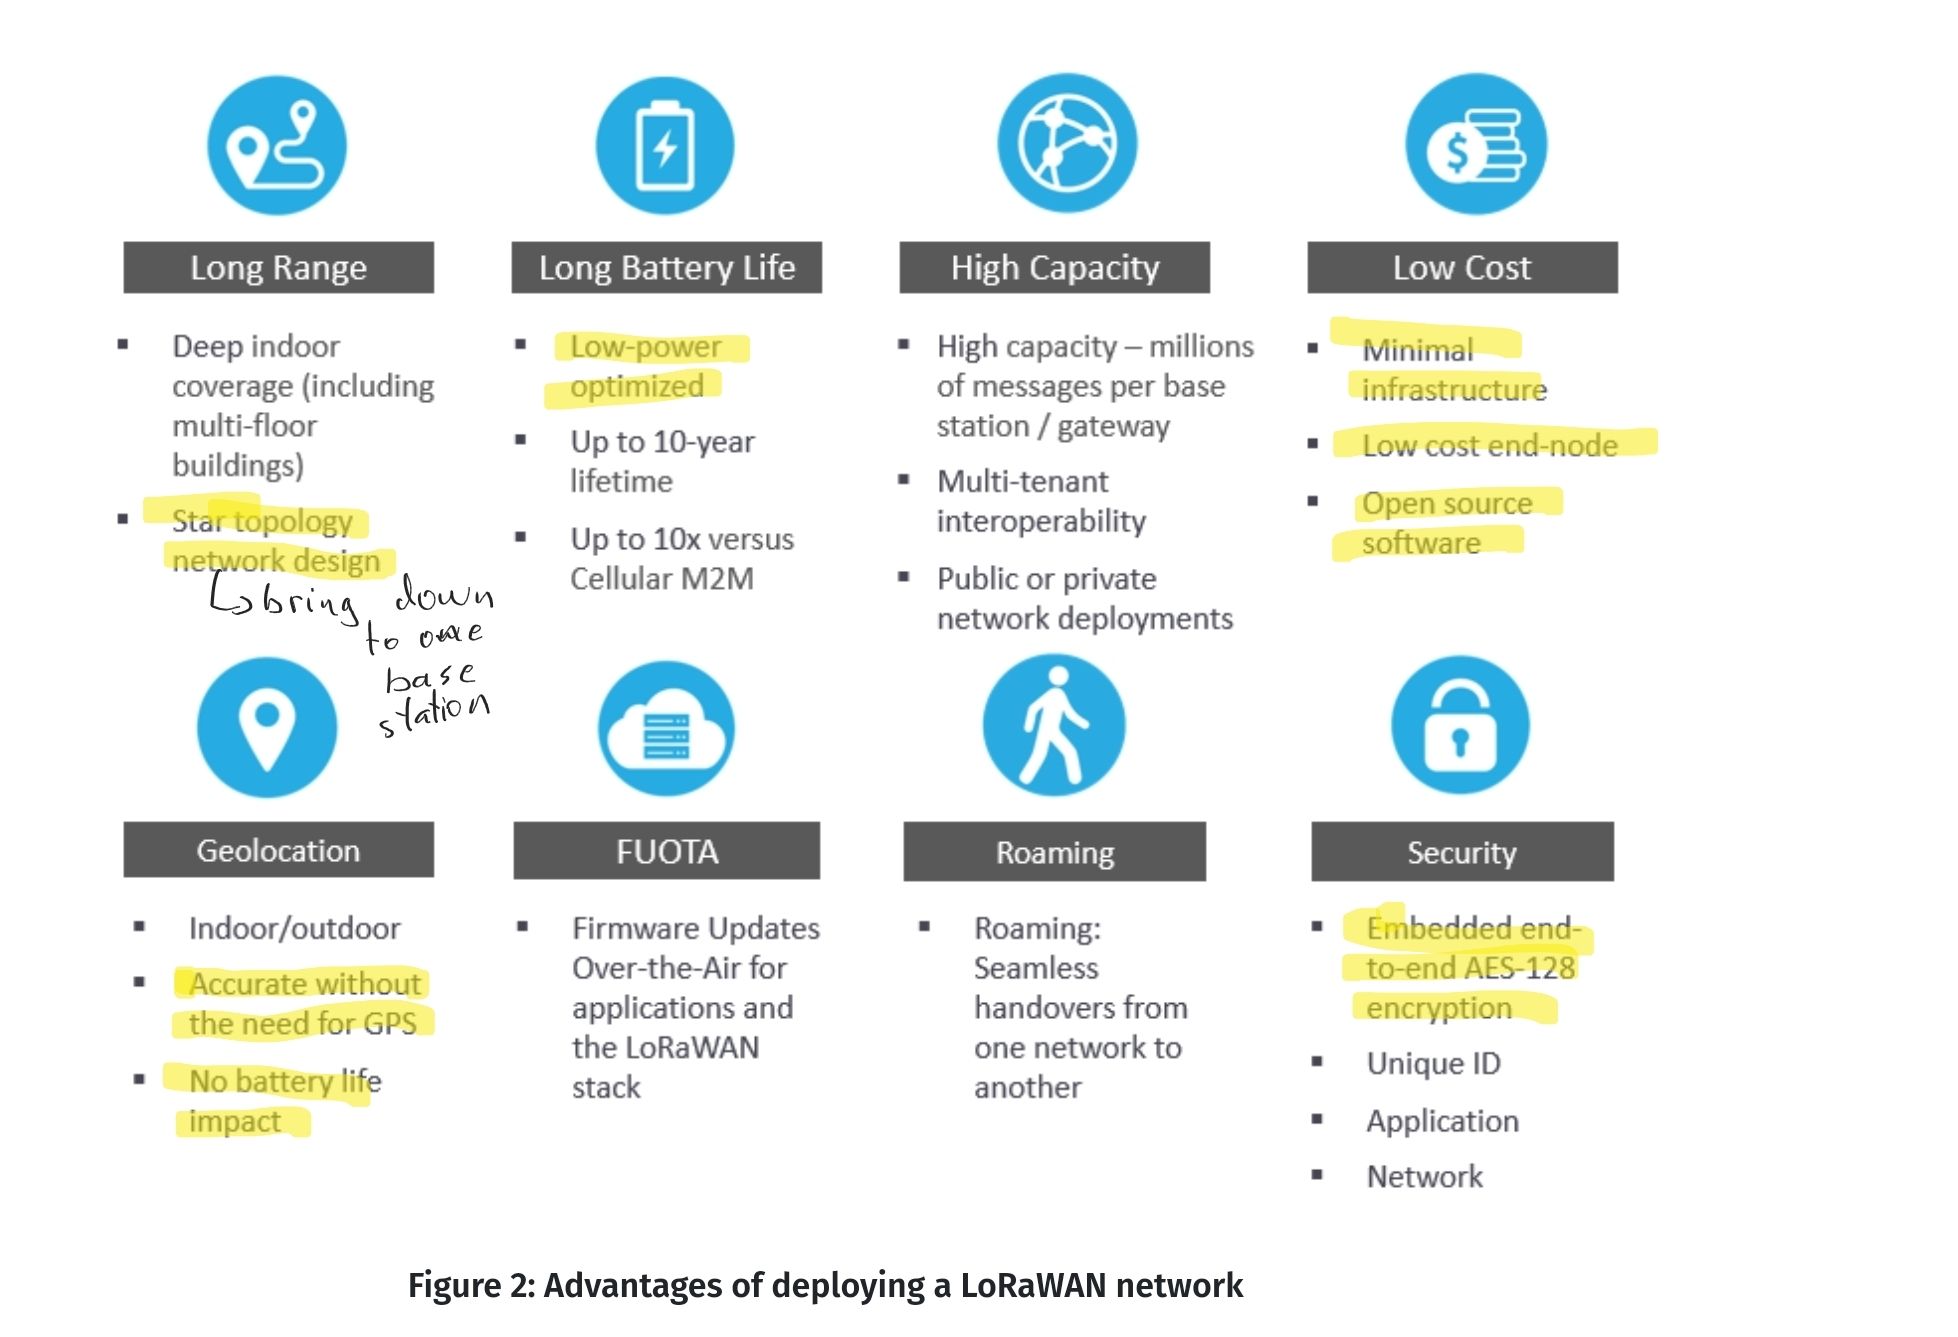
\includegraphics[scale=0.15]{Advantages-deploying-lora.jpg}
  \end{center}
\end{frame}

\begin{frame}[t]
  \frametitle{Reference }
  \framesubtitle{Sources}
 \begin{itemize}
    \item \url{https://www.youtube.com/watch?v=ciL0MOtm50A&t=118s&ab_channel=MilesightIoT}{LORAWAN}
    \item \url{https://wiki.seeedstudio.com/WM1302_Pi_HAT/}{Pi HAT}
  \end{itemize}
\end{frame}


\end{document}
